\section{Neural Network}

The Convolutional Auto-Encoder is used to de-noise raw data from CLAS12 drift chambers~\cite{Thomadakis:2022zcd}. The input and output for the network are 
matrices of size 36x112 representing hits in one sector of drift chambers. 
The training data was extracted from experimental data. The raw hits (converted 
into a matrix) were used as an input for the neural network and a matrix constructed 
only from hits that belong to reconstructed tracks an output (see Figure~\ref{conv:trackfinding}). 
In training data set multiple track hits were allowed in the output matrix. The structure 
of neural network can be seen on Figure~\ref{network:cnn_encoder}.

\begin{figure}[!h]
\begin{center}
 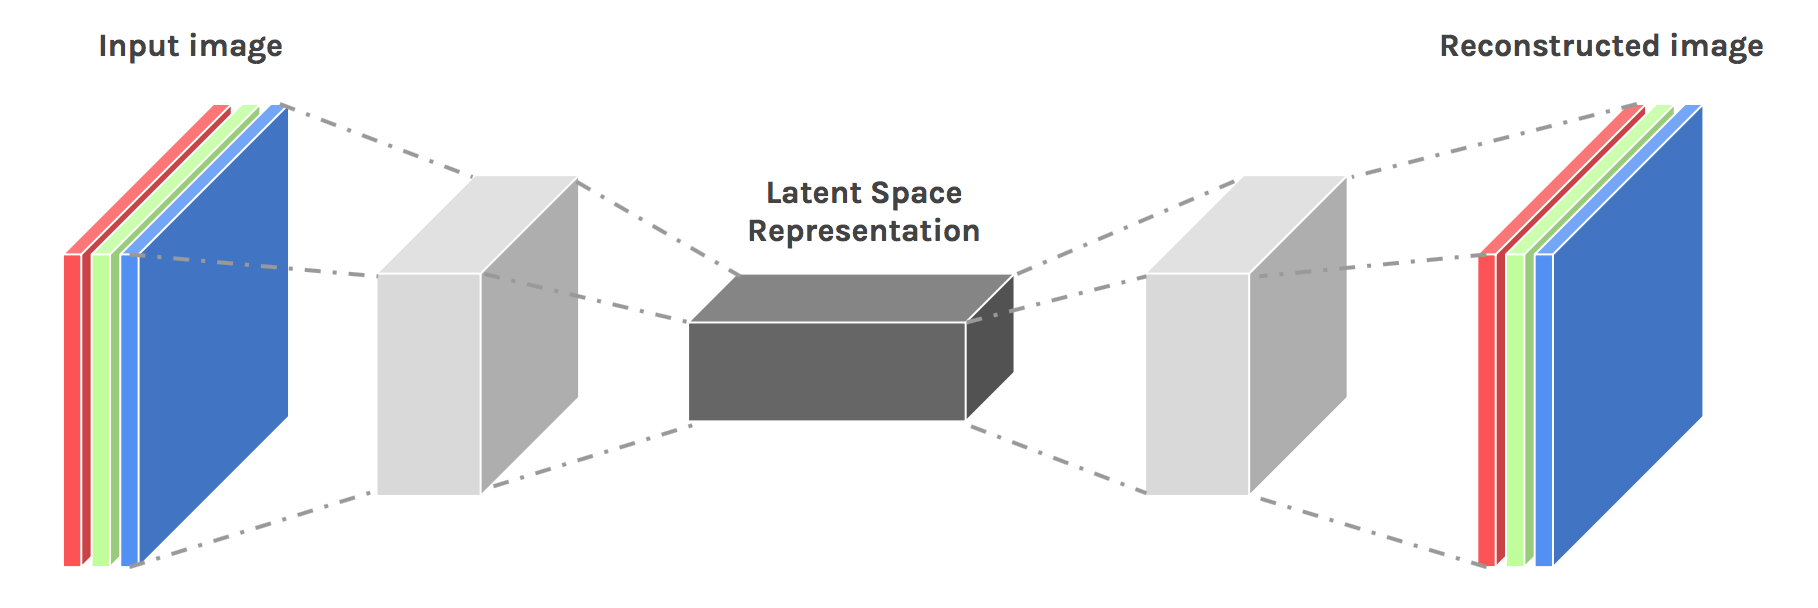
\includegraphics[width=5.1in]{images/convolutional-autoencoder.png}
\caption {De-noising Convolutional Auto-Encoder architecture. }
 \label{network:cnn_encoder}
 \end{center}
\end{figure}

The network was validated on experimental data where number of hits along the 
track trajectory were compared for de-noised data. Example of comparison can 
be seen in Figure~\ref{network:cnn_results} where raw data (left column) is shown 
along with data with hits belonging to reconstructed track (middle column) and 
reduced data passing through de-nosing program (right column).

\begin{figure}[!h]
\begin{center}
 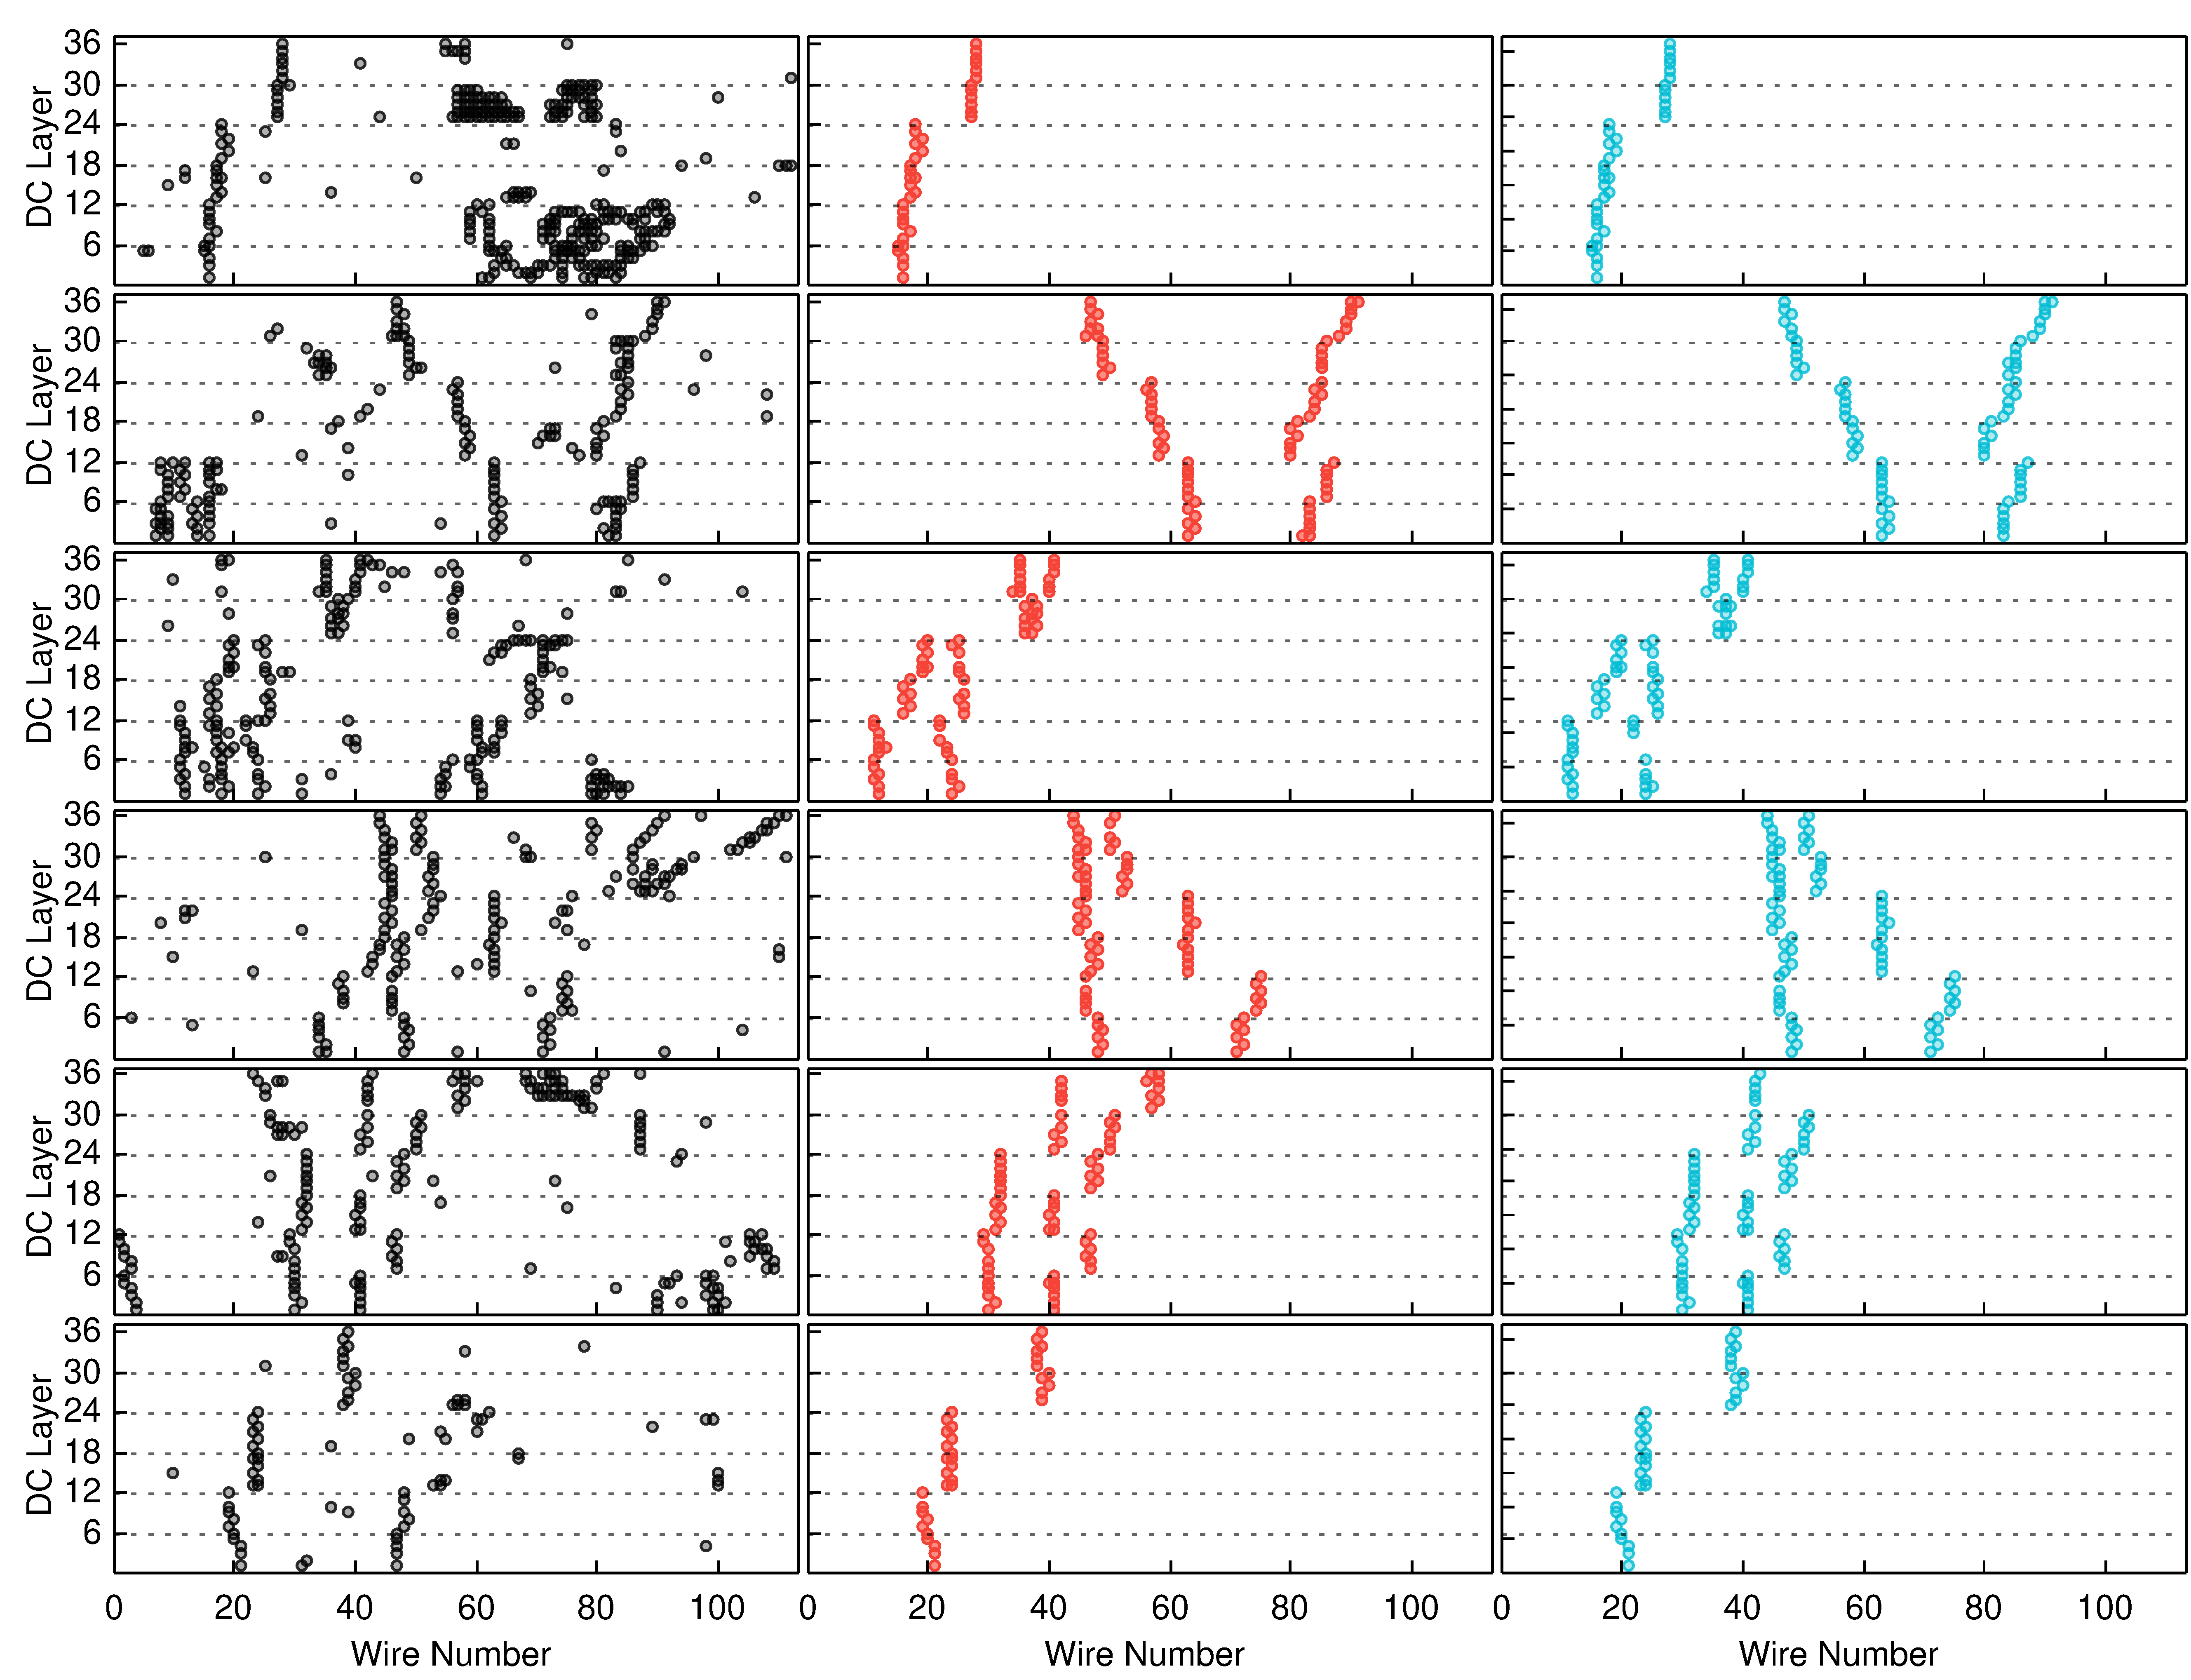
\includegraphics[width=5.8in]{images/cnn_denoise_results.pdf}
\caption {Results from de-noising auto-encoder. The raw signal hits are shown
in the left column for 5 random events, along with hits reconstructed by the 
CLAS12 tracking algorithm in the middle column. The resulting  hits matrix 
from de-noising raw hits are shown in the right column. (Systematic studies 
of de-noiser performance can be found here~\cite{Thomadakis:2022zcd})}
 \label{network:cnn_results}
 \end{center}
\end{figure}

As can be seen from the figure de-noiser removes all background hits not associated 
with a track. Systematic studies~\cite{Thomadakis:2022zcd} showed that more than 
$95\%$ of the track related hits are preserved in the output of de-noiser while 
background hits are significantly suppressed for normal experimental conditions of 45nA
incident beam current. Systematic studies showed that in more than $85\%$ of cases all 
6 clusters belonging to the track are fully identified by the algorithm after de-noising, 
and $>97\%$ of the cases 5 clusters from the original track are recovered. The CLAS12 
track reconstruction algorithm can reconstruct tracks with only 5 clusters along the 
track trajectory, which means that even if some clusters are lost due to de-noising procedure 
the track efficiency does not suffer significantly from this.

For out implementation we used TensorFlow/Keras~\cite{keras-website} to train 
and evaluate the network. The resulting network parameters (weights) were saved 
in HDF5 file. The de-noiser implementation for CLAS12 reconstruction software is 
done using DeepLearning4J~\cite{dl4j-website} which supports model imports 
through HDF5 files. The de-noising is not yet implemented as a part of CLAS12 
reconstruction workflow, and works as a standalone package to process raw data 
before analyzing with reconstruction software.
